\documentclass{beamer}
\usetheme{Madrid}
\usepackage{amsmath, amssymb, bm}
\usepackage{tcolorbox}
\usepackage{tikz}
\usepackage{tikz-cd}

% Aggiungi questa linea per risolvere il problema di tikz-cd in beamer
\tikzcdset{ampersand replacement=\&}

% Box styles
\tcbset{
    myformula/.style={colback=blue!5!white, colframe=blue!75!black, sharp corners, boxrule=0.8pt, left=2mm, right=2mm, top=1mm, bottom=1mm},
    myexample/.style={colback=green!5!white, colframe=green!75!black, sharp corners, boxrule=0.8pt, left=2mm, right=2mm, top=1mm, bottom=1mm},
    mynote/.style={colback=yellow!5!white, colframe=yellow!75!black, sharp corners, boxrule=0.8pt, left=2mm, right=2mm, top=1mm, bottom=1mm}
}

\title{Parametric Sensitivity in Optimization}
\author{}
\date{}

\begin{document}

\frame{\titlepage}

%------------------------------------------------
\begin{frame}{Problem Setup}
Consider a parametric optimization problem:
\[
\min_{x \in \mathbb{R}^n} f(x,p), \quad p \in \mathbb{R}^m
\]

\textbf{Goal:} Determine how $x^*(p)$ changes with $p$.

\textbf{Applications:}
\begin{itemize}
    \item Sensitivity analysis
    \item Warm-starting solvers
    \item Gradient-based optimization over parameters
\end{itemize}
\end{frame}

%------------------------------------------------
\begin{frame}{Unconstrained Optimization: Sensitivity}
Optimality condition:
\[
\nabla_x f(x^*(p),p) = 0
\]

Differentiate w.r.t $p$:
\[
\frac{d}{dp}\nabla_x f(x^*(p),p) = 0
\implies \nabla^2_{xx} f \frac{\partial x^*}{\partial p} + \nabla^2_{xp} f = 0
\]

\begin{tcolorbox}[title=Sensitivity Formula, myformula]
\[
\frac{\partial x^*}{\partial p} = - (\nabla^2_{xx} f)^{-1} \cdot \nabla^2_{xp} f
\]
\end{tcolorbox}

\textbf{Interpretation:}
\begin{itemize}
    \item Each column: sensitivity of $x^*$ to $p_j$
    \item Each row: sensitivity of $x_i^*$ to all parameters
\end{itemize}
\end{frame}

%------------------------------------------------
\begin{frame}{Unconstrained: Matrix Visualization}
\begin{center}
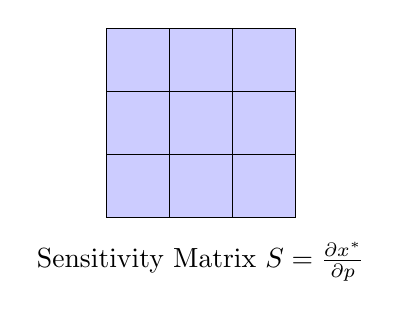
\begin{tikzpicture}[scale=0.8]
% Sensitivity matrix
\foreach \i in {0,1,2} {
    \foreach \j in {0,1,2} {
        \draw[fill=blue!20] (\j,\i) rectangle (\j+1,\i+1);
    }
}
\node at (1.5,-0.7) {Sensitivity Matrix $S = \frac{\partial x^*}{\partial p}$};
\end{tikzpicture}
\end{center}
\end{frame}

%------------------------------------------------
\begin{frame}{Box Constraints: KKT Conditions}
\[
\nabla_x f(x^*,p) + \lambda = 0
\]

\[
\lambda_i \ge 0 \text{ if } x_i^* = l_i, \quad
\lambda_i \le 0 \text{ if } x_i^* = u_i, \quad
\lambda_i = 0 \text{ if } l_i < x_i^* < u_i
\]

\textbf{Active / Free sets:}
\[
F = \{ i: l_i < x_i^* < u_i \}, \quad
A = \{ i: x_i^* \text{ at bounds} \}
\]
\end{frame}

%------------------------------------------------
\begin{frame}{Active / Free Set Visualization}
\begin{center}
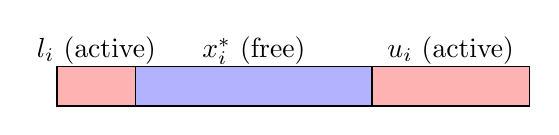
\begin{tikzpicture}[scale=1]
\draw[thick] (0,0) -- (6,0);
\draw[fill=red!30] (0,0) rectangle (1,0.5); \node at (0.5,0.7){$l_i$ (active)};
\draw[fill=blue!30] (1,0) rectangle (4,0.5); \node at (2.5,0.7){$x_i^*$ (free)};
\draw[fill=red!30] (4,0) rectangle (6,0.5); \node at (5,0.7){$u_i$ (active)};
\end{tikzpicture}
\end{center}
\end{frame}

%------------------------------------------------
\begin{frame}{Sensitivity with Box Constraints}
For free variables $i \in F$:
\[
H_{FF} \cdot \left(\frac{\partial x^*}{\partial p}\right)_F = - G_F
\]

For active variables $i \in A$:
\[
\frac{\partial x_i^*}{\partial p} = 0
\]

\begin{tcolorbox}[title=Discontinuity Warning, mynote]
$x^*(p)$ is not differentiable when the active set changes.
Example: $\min (x-p)^2 \text{ s.t. } x \le 1$:
\[
x^*(p) = \begin{cases} p & p \le 1 \\ 1 & p > 1 \end{cases}, \quad
\frac{dx^*}{dp} = \begin{cases} 1 & p<1 \\ 0 & p>1 \end{cases}
\]
\end{tcolorbox}
\end{frame}

%------------------------------------------------
\begin{frame}{Flowchart: Active Set Changes}
\begin{center}
% Usa \& invece di & nel diagramma tikz-cd
\begin{tikzcd}[row sep=2em, column sep=3em, ampersand replacement=\&]
p \text{ changes} \arrow[r] \& 
\text{Check } x^*(p) \text{ vs bounds} \arrow[r, "{\text{Active set changes?}}"] \& 
\text{Yes} \arrow[d, "{\text{update } F,A}"] \\
\& \& 
\text{No} \arrow[d, "{\text{S unchanged}}"'] \\
\& \& 
\text{Compute } S_F = -H_{FF}^{-1} G_F
\end{tikzcd}
\end{center}
\end{frame}

%------------------------------------------------
\begin{frame}{L2-Regularized Problem (Centered)}
\[
\min f(x,p) + \varepsilon \|x - x_0\|^2
\]

\textbf{Note:} $x_0$ is a reference/center point (e.g., prior guess, warm start).

Optimality condition:
\[
\nabla_x f(x^*,p) + 2 \varepsilon (x^* - x_0) = 0
\]

\begin{tcolorbox}[title=Regularized Sensitivity (Centered), myformula]
\[
\frac{\partial x^*}{\partial p} = - (\nabla^2_{xx} f + 2 \varepsilon I)^{-1} \cdot \nabla^2_{xp} f
\]
\end{tcolorbox}

\textbf{Effects:}
\begin{itemize}
    \item Same formula as before! (Hessian modification unchanged)
    \item Regularization pulls solution toward $x_0$
    \item Better conditioning, reduced sensitivity, smoother $x^*(p)$
\end{itemize}
\end{frame}

%------------------------------------------------
\begin{frame}{Why the Same Formula?}
For $\min f(x,p) + \varepsilon \|x - x_0\|^2$:

Optimality:
\[
\nabla_x f(x^*,p) + 2\varepsilon(x^* - x_0) = 0
\]

Differentiate w.r.t $p$:
\[
\nabla^2_{xx} f \cdot \frac{\partial x^*}{\partial p} + \nabla^2_{xp} f + 2\varepsilon I \cdot \frac{\partial x^*}{\partial p} = 0
\]

Rearrange:
\[
(\nabla^2_{xx} f + 2\varepsilon I) \frac{\partial x^*}{\partial p} = - \nabla^2_{xp} f
\]

\begin{tcolorbox}[myexample]
\textbf{Key insight:} $x_0$ disappears after differentiation because $\frac{\partial}{\partial p}(x_0) = 0$ (reference point is fixed).
\end{tcolorbox}
\end{frame}

%------------------------------------------------
\begin{frame}{Visualizing Sensitivity Matrices}
\begin{center}
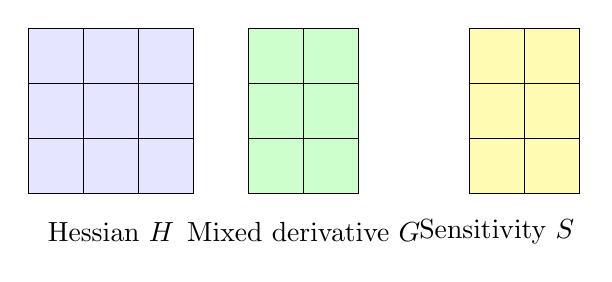
\begin{tikzpicture}[scale=0.7]
% Hessian H
\foreach \i in {0,1,2} {
    \foreach \j in {0,1,2} {
        \draw[fill=blue!10] (\j,\i) rectangle (\j+1,\i+1);
    }
}
\node at (1.5,-0.7) {Hessian $H$};

% Mixed derivative G
\foreach \i in {0,1,2} {
    \foreach \j in {0,1} {
        \draw[fill=green!20] (4+\j,\i) rectangle (5+\j,\i+1);
    }
}
\node at (5,-0.7) {Mixed derivative $G$};

% Sensitivity S
\foreach \i in {0,1,2} {
    \foreach \j in {0,1} {
        \draw[fill=yellow!30] (8+\j,\i) rectangle (9+\j,\i+1);
    }
}
\node at (8.5,-0.7) {Sensitivity $S$};
\end{tikzpicture}
\end{center}
\end{frame}

%------------------------------------------------
\begin{frame}{Practical Implementation Steps}
\begin{enumerate}
    \item Solve $\min f(x,p) + \varepsilon\|x-x_0\|^2$ to get $x^*(p)$
    \item Compute $H = \nabla^2_{xx} f$, $G = \nabla^2_{xp} f$
    \item If regularized: $H \leftarrow H + 2\varepsilon I$
    \item Identify active set $A$, free set $F$ (for constrained case)
    \item Solve $H_{FF} S_F = - G_F$
    \item Construct full sensitivity $S$: $S[i]=S_F[k]$ if $i\in F$, else $0$
\end{enumerate}
\end{frame}

%------------------------------------------------
\begin{frame}{Applications}
\begin{itemize}
    \item Warm-starting: $x^*(p_\text{new}) \approx x^*(p_\text{old}) + S \Delta p$
    \item Sensitivity analysis: identify influential parameters
    \item Gradient-based optimization: $\frac{\partial f_\text{opt}}{\partial p} = \nabla_p f(x^*,p)$
    \item Optimal control / MPC: fast parametric gradients
    \item Bayesian inference: $\|x-x_0\|^2$ as Gaussian prior
\end{itemize}
\end{frame}

\end{document}